\documentclass{article}
\usepackage{float,amsmath}
\usepackage{graphicx}
\usepackage{color}
\usepackage[letterpaper,margin=1in]{geometry}
\usepackage{hyperref}

%\setlength{\textwidth}{6.5in}

\begin{document}

\author{David DeBoer}
\title{Array Configuration Management Database}
\maketitle

\section{Introduction}
The HERA array/part configuration management database is a set of five tables within the larger hera\_mc database, which is maintained on-site in the Karoo.  The tables are detailed in the Appendix, 
but they are:  
\begin{tabular}{l l l}
         {\bf psql table} & {\bf python file}  &  {\bf class name} \\
	geo\_location 	& hera\_mc/geo\_location.py & GeoLocation \\
	station\_meta 	& hera\_mc/geo\_location.py & StationMeta \\
	parts\_paper 	& hera\_mc/part\_connect.py & Parts \\
	part\_info 	         & hera\_mc/part\_connect.py & PartInfo \\
	connections 	& hera\_mc/part\_connect.py & Connections \\
\end{tabular}

Software is contained in the repository https://github.com/HERA-Team/hera\_mc.

The databases are structured primarily around {\em parts} and {\em connections}.  {\em Parts} are meant to be single items that, in theory at least, are a thing than can be replaced as a unit.  
{\em Connections} define {\em ports} on a given {\em part} and connect two {\em ports} together.  All {\em parts} and {\em connections} are timed in that they have a start and stop time of operation.  If stop is {\tt None}, then it is active (it is given a date in the relatively far future).  There are currently two special parts (one at each end of the signal chain):
\begin{itemize}
	\item {\bf geo\_location}: a geo\_located part (``station'') is a named location with UTM coordinates which also has an entry in the geo\_location table;
	\item {\bf f\_engine}:  each input to the f\_engine ROACH-2 is currently listed as a separate part.  Probably it should be a 32-input part, but given timing will wait for the new architecture.
\end{itemize}

Parts are hooked together via connections of their ports.   For parts in the PAPER era, the signal chain hook-up is given below and shown in Fig. \ref{fig:hookup}.
\begin{itemize}
\setlength\itemsep{-.3em}
	\item {\bf Station}: geo\_located position.  See prefixes in table station\_meta
	\item {\bf Antenna}:  collecting element ({\em this used as the correlator number,} {\tt \{C\}}):  {\tt{\bf A}\{C\}}
	\item {\bf Feed}:  element feed.  {\tt {\bf FDP}\{\#\}} are PAPER feeds, {\tt {\bf FDA}\{\#\}} are design A HERA feeds.
	\item {\bf Frontend}:  lna, etc at feed.  {\tt {\bf FEA}\{\#\}} is design A (75 $\Omega$)
	\item {\bf Cable\_feed75}:  cable from front-end to receiverator: {\tt {\bf C7F}\{\#\}}
	\item {\bf Cable\_receiverin}:  cable inside {\tt R}$^{th}$ receiverator to receiver: {\tt {\bf RI}\{R\}\{"A"/"B"\}\{\#\}\{"E"/"N"\}}
	\item {\bf Receiver}:  receiver module in receiverator: {\tt {\bf RCVR}\{SN\}}
	\item {\bf Cable\_receiverout}:  cable inside receiverator from receiver {\tt {\bf RO}\{R\}\{"A"/"B"\}\{\#\}\{"E"/"N"\}}
	\item {\bf Cable\_receiverator}:  cable from receiverator to container {\tt {\bf CR}\{R\}\{"A"/"B"\}\{\#\}\{"E"/"N"\}}
	\item {\bf Cable\_container}:  cable inside container from {\tt\{P\}}late/{\tt\{Row\}}/{\tt\{Col\}}umn {\tt {\bf CC}\{P\}{\bf R}\{Row\}{\bf C}\{Col\}}
	\item {\bf F\_engine}:  {\tt\{R2\}} Roach-2 input {\tt {\bf DF}\{R2\}\{"A"-"H"\}\{\#\}}
\end{itemize}

In the hook-up listing (using the -m flag), the Antenna number (without the {\tt A}) is also displayed under the station just to help the user find the antenna number that the correlator cares about.  It maps antenna to position to correlator input.

\begin{figure}[H]
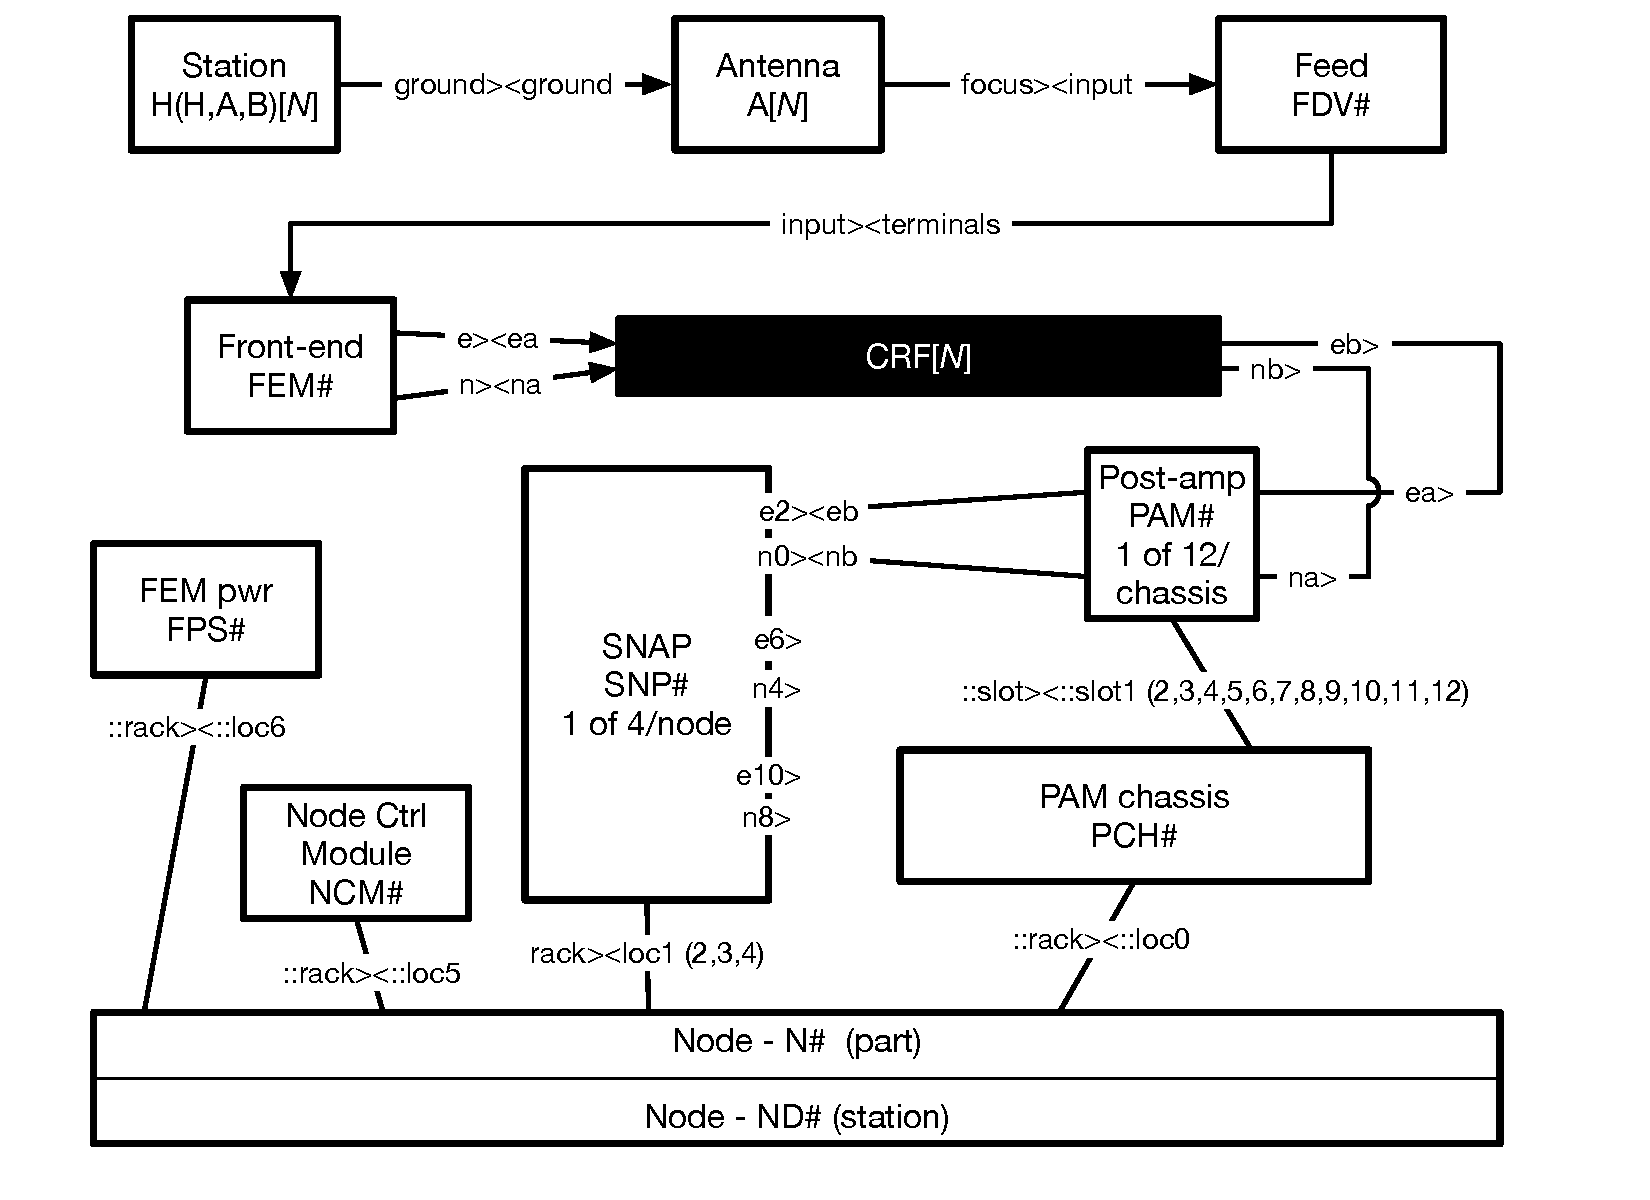
\includegraphics[width=0.8\textwidth]{hookup.pdf}
\centering
\caption{Block diagram of hookup.  Filled boxes are cables, blue objects are in the receiverator and green objects are in the container.
The line labels indicate the port names/connections.}
\label{fig:hookup}
\end{figure}

2. Use Cases
Three use cases are identified:
In-the-field
Remote user
Bulk database
2.1. In-the-field updates
This is the ?operational? mode, where inputs to the on-site database are done via scripts (command-line and/or web), which update the database directly.  These scripts will be documented under the repository software.
2.2. Remote user
Remote use is the case when a remote user initializes and uses the tables outside of the main database.  This assumes that postgresql etc is configured on the remote computer.  Note that this mode supports both offline use (essentially steps 3-5 below, which are in bold) and development (probably all steps).  The process is as follows: 
Generate ascii files of the tables in the main database (in the Karoo)
      	(cm\_package.py [--tables table1,table2,...)
Push to GitHub
Pull down to remote computer
Install (python setup.py install, although not necessarily needed)
Initialize the updated ones (cm\_initialize.py)
If you are developing, make a base version before you start
(cm\_package.py --base)

Note that generally you should leave off the --tables option, since you should use all the tables so as to not break foreign keys (it is left there for ?expert? users).  Steps 3-5 are bolded, since if you just want to pull down the latest and use it assuming things are up-to-date they are all that are needed (i.e., leave the ?packaging to the experts?).
	This has another option of --base, so that you can set up a base copy to which you can revert if need be by including --base on both commands (step 6).
2.3. Main database updates
This is effectively the opposite of the remote user case, bringing an updated set of table(s) back into the main database.  The process is as follows:
Generate ascii files of the desired tables from the remote database: 
(cm\_package.py --maindb $key [--tables table1,table2,...])
Push to GitHub
Pull down to site computer
Install
Update existing tables 
(cm\_initialize.py --maindb $key [--tables table1,table2,])
As per above, you should generally leave off the --tables option so as to do them all.  You should be sure it all works on the remote computer by running the pair of commands
cm\_package.py
cm\_initialize.py 
and leave off the --maindb $key, which is only needed for updating the site main database.  The --base would also work for the main database, but would also require --maindb $key, which you?d have to remember or look up to reapply the base.

%4. Tables
%
%The configuration management database comprises the following tables:
%
%Column
%Type 
%Description
%geo_location :: geo_location.GeoLocation
%station_name*
%character varying(64)
%Name of position - never changes
%station_type_name*(1)
%character varying(64)
%Type of station
%datum
%character varying(64)
%UTM datum
%tile
%character varying(64)
%UTM tile
%northing
%double precision
%UTM coordinate
%easting
%double precision
%UTM coordinate
%elevation
%double precision
%Elevation
%created_date*
%datetime
%Date and time of creation.
%geo_location :: station_type.StationType (was station_meta:StationMeta)
%station_type_name*(1)
%character varying(64)
%Station type name
%(was meta_class_name)
%prefix*
%character varying(64)
%1-2 letter prefix for part station_name
%description
%character varying(64)
%Short description
%plot_marker
%character varying(64)
%Type of matplotlib marker
%part_connect :: parts_paper.Parts
%hpn*(2)
%character varying(64)
%HERA part number
%hpn_rev*(3)
%character varying(32)
%HPN revision letter (A-Z)
%hptype*
%character varying(64)
%HPN part type category
%manufacturer_number
%character varying(64)
%Unique serial number for each part
%start_date*
%timestamp no time zone
%Datetime when part/rev is activated.
%stop_date
%timestamp no time zone
%Datetime when part/rev is de-activated
%part_connect :: part_info.PartInfo
%hpn*(2)
%character varying(64)
%HERA part number
%hpn_rev*(3)
%character varying(32)
%HPN revision letter (A-Z)
%posting_date*
%timestamp no time zone
%Date information was posted
%comment*
%character varying(1024)
%Comment
%library_file
%character varying(256)
%Librarian filename (how to get it there?)
%(was info)
%part_connect :: connections.Connections
%upstream_part*(2)
%character varying(64)
%Hera part number of upstream connection
%(was up)
%up_part_rev*(3)
%character varying(32)
%Hera part revision of upstream connection
%(was up_rev)
%downstream_part*(2)
%character varying(64)
%Hera part number of downstream connection
%(was down)
%down_part_rev*(3)
%character varying(32)
%Hera part revision of downstream connection
%(was down_rev)
%upstream_output_port*
%character varying(64)
%Output port on upstream part
%(was b_on_up)
%downstream_input_port*
%character varying(64)
%Input port on downstream part
%(was a_on_down)
%start_date*
%timestamp with time zone
%Date when connection started
%stop_date
%timestamp no time zone
%Date when connection ended
%Bold 	= primary_key
%Italics(#)	= foreign_key, defining if underlined, # identifies locations, can be bold
%           *  	=  NotNull
%
%
%


\end{document}